We considered how to display links explicitly on the mobile screen. It might be tempting simply to draw lines between linked nodes (Figure \ref{fig:linkrep}c), but \textit{GraphTiles} has unique characteristics that could make this solution untenable. As users scroll, nodes appear and disappear, meaning that linking lines do as well. Scrolling also causes the lines to move when they are onscreen, occluding a variety of other nodes and dynamically relocating link crossings (making a well-known drawback of link lines still worse). All of this dynamic behavior does not exist in most graph visualizations and could be quite disorienting during mobile search. .

In creating alternative designs for displaying explicit links, we were (loosely) inspired by the grouping principles of Gestalt psychology ~\cite{RefWorks:562}. The \textit{proximity} principle places nearby items in the same group. Because we could not use proximity alone to display complex many-to-many relationships, we approximated proximity with an iconic representation of the neighboring column (Figure \ref{fig:linkrep}(d)). Rectangles in the representation indicate the presence of links to the node in the same position in the neighboring column. \textit{Similarity} groups items that have similar properties such as color or texture (Figure \ref{fig:linkrep}(b) and \ref{fig:linkrep}(e)). Here, nodes containing the outline color or a thumbnail of a neighboring node are linked to that node. Like link lines (which use the Gestalt principle of \textit{connectedness}), all of these representations must dynamically change as the user scrolls and nodes move, but the changes are much more restrained.

\begin{figure*}[htb!]
\centering
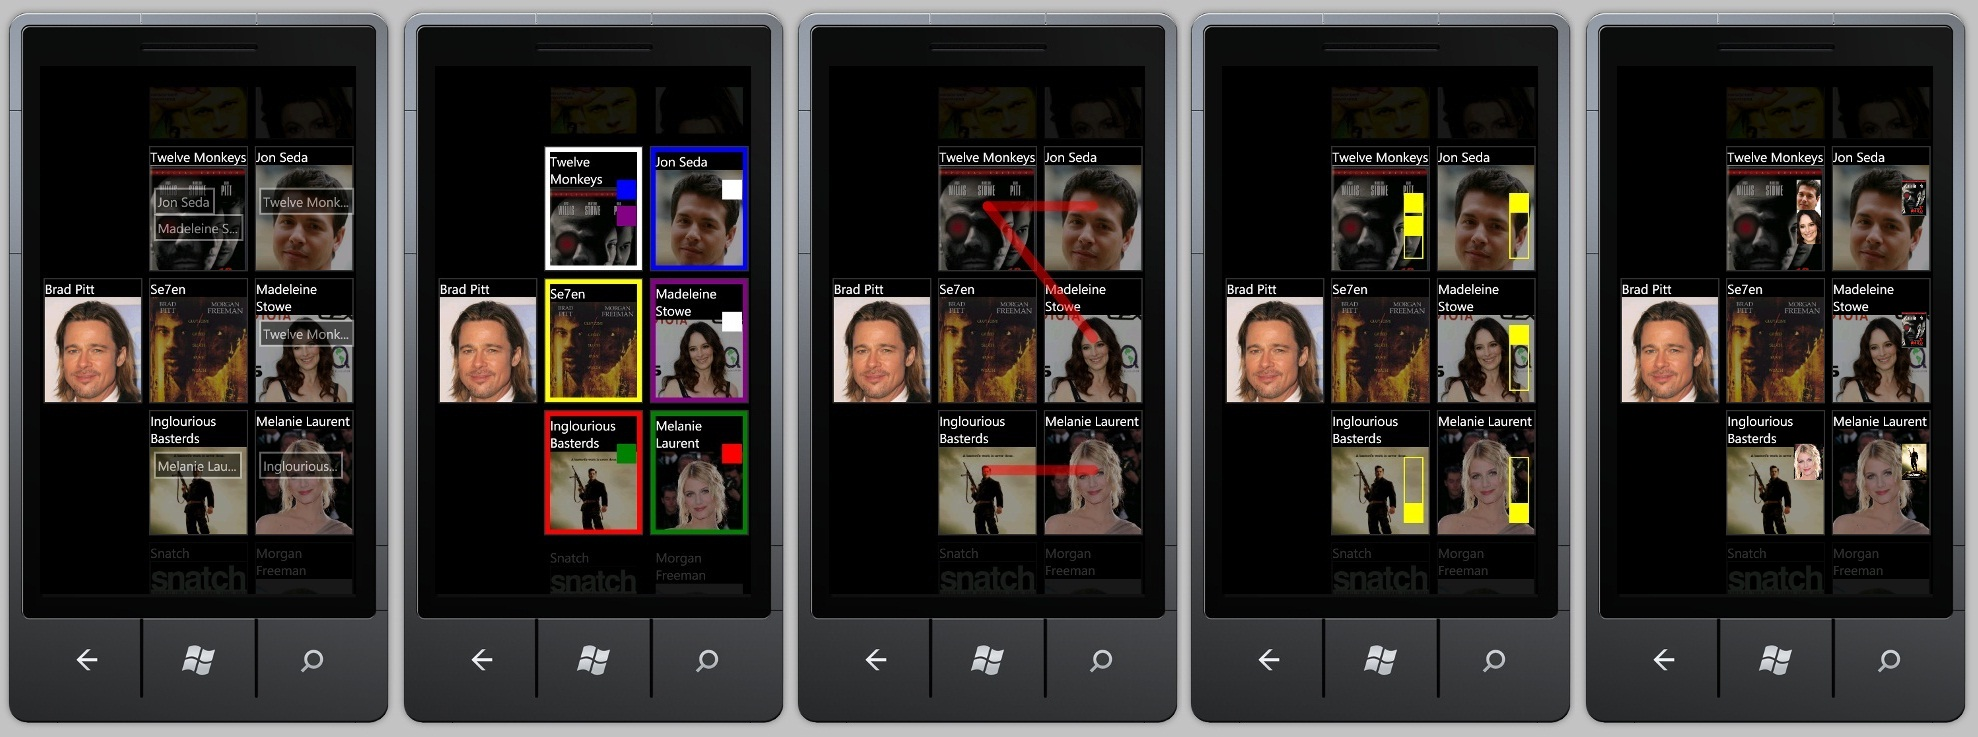
\includegraphics[width=7in]{images/linkrep}
\caption{Different explicit link representations for \textit{GraphTiles}. (a) \emph{text:} nodes with the same name are linked. (b) \emph{color:} nodes with the same color are linked. (c) \emph{connectedness:} nodes with lines between them are linked. (d) \emph{proximity:} nodes at/containing the same vertical position are linked. (e) \emph{texture:} nodes with/containing the same image are linked.}
\label{fig:linkrep}
\end{figure*}

\subsection{Method}

Using IMDb as a testbed, we compared connectedness-inspired lines to our alternative designs in a controlled experiment, and included a text-based link display (Figure \ref{fig:linkrep}(a)) as a control condition. In this condition, nodes with the same text were linked. Note that because we were testing only explicit link representations, we did not enable interactive reordering in this experiment.

We expected that connectedness-, color- and texture-inspired links would perform better than text-based or proximity-inspired links. Because of the unique dynamic qualities of the \textit{GraphTiles} visualization, we did not attempt to predict which link representation would be best.

\subsubsection{Design}

We used a fully crossed within subjects $5 \times 2 \times 2$ design. Link \textit{Depiction} had five levels: text-based as well as proximity-, color-, texture-, and connectedness-inspired representations. \textit{QueryType}, or the type of question asked, had two levels: a movie-person-movie (MPM) query or a person-movie-person (PMP) query. \textit{Size}, or the rough size of the surrounding graph neighborhood, had two levels: small or below median, and large or above median.


\subsubsection{Participants and Procedure}

We had ten participants, all university students with normal or corrected-to-normal vision. We obtained informed consent from the participants, and asked them to read the instructions for the experiment. We then familiarized them with the task and link depictions using 10 training datasets, one for each combination of link \textit{Depiction} and \textit{QueryType}. Participants were free to ask verbal questions during training.

Participants then each performed $120$ information seeking tasks, each using a different graph neighborhood in the IMDb database, with median size of 115 nodes. On average, they completed all their tasks in one hour. Every participant performed six trials with each of the $5 \times 2 \times 2 = 20$ experimental treatments. We formed five blocks of $24$ trials each, each block corresponding to one \textit{Depiction}. Thus participants performed all trials with the current \textit{Depiction} before moving on to the next. To combat the effects of fatigue and learning, we sampled all the orderings of \textit{Depiction} using a $5 \times 5$ Latin Square. Within each of these \textit{Depiction} blocks, we formed two 12-trial \textit{QueryType} blocks. Half of the participants performed MPM questions first, half performed PMP questions first. Within each \textit{QueryType} block, participants performed 6 trials with small neighborhoods and 6 with large neighborhoods. We randomized the order of these trials. To avoid any confound between treatments and graph neighborhoods, we randomized the match of graph to treatment. Each participant saw each neighborhood only once.

For each task, participants answered a question displayed on a nearby monitor. 
As for the \textit{QueryType}, we used the same method as the previous summative experiment.
We recorded the time to complete each trial, and whether or not the participant performed the trial correctly. Participants were paid \$10 for their effort.


\subsection{Results}
\begin{figure}[ht]
\centering
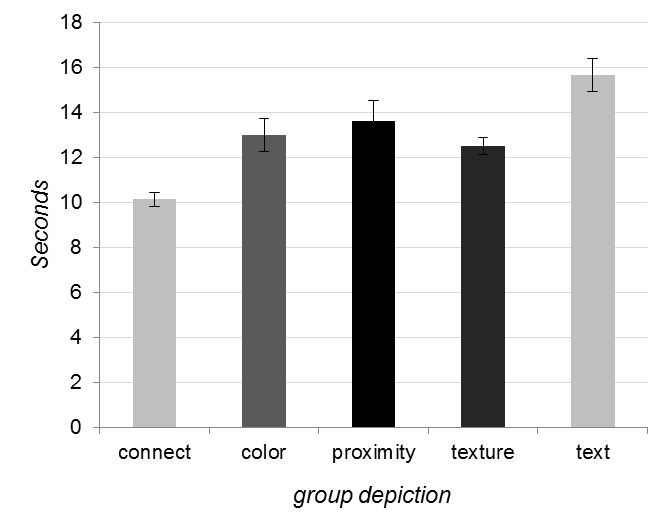
\includegraphics[width=3in]{images/depictiongraph}
\caption{Average task completion times per depiction for the first experiment.}
\label{fig:experiment1}
\end{figure}

All participants completed all trials correctly, so we report only on completion time here. On completion times, we performed a single, three-factor repeated measures ANOVA. All single variable effects were significant. 

The connectedness-inspired link Depiction indeed supported the fastest information seeking performance ($F(4,36)=4.942, p<0.005$). Average completion times in seconds for each Depiction were: connectedness $10.1$s, texture $12.5$s, color $13.0$s, proximity $13.6$s, and text $15.7$s. We show the same times in Figure \ref{fig:experiment1}, along with standard error. Despite their drawbacks, link lines also have strengths: they are familiar to most viewers;  and they are simple, introducing only one primitive per link, while other representations require changes at both linked nodes.


Participants were much faster when asked to locate a person (the MPM \textit{QueryType}) than when asked to locate a movie (PMP) ($F(1,9)=43.869, p<0.001$). Average completion times for person queries were 10.5s, and for movies 15.5s. This is likely an effect of graph size rather than some more subtle task difference. Recall that IMDb's API returned many more top actors working on a movie than top movies in which an actor worked. This meant that PMP neighborhoods contained many more nodes than MPM neighborhoods.

Participants were faster when working with small graph Sizes than with large graph Sizes ($F(1,9)=83.911, p<0.001$). Average completion times for small graphs were $11.7$s, while for large graphs they were $14.2$s.

The only significant interaction occurred between the \textit{QueryType} and \textit{Size} variables ($F(1,9)=25.824, p=0.001$). When participants were asked to find movies in PMP neighborhoods, increasing graph Size had a large effect on completion times ($13.4$s vs. $17.6$s). When they were asked to find persons in MPM neighborhoods, \textit{Size}'s effect was minor ($10.1$s vs. $10.9$s). In PMP neighborhoods, graphs were larger, so increasing \textit{Size} had a larger effect.

Readers may wonder why average times in this experiment with \textit{GraphTiles} were lesser than they were in our first experiment. One cause may be the increased practice with \textit{GraphTiles} (10 training datasets) in this experiment.


\subsection{Discussion}
Results largely matched our expectations, with text-based and proximity-inspired links performing worst, texture- and color- inspired link \textit{Depictions} performing better, and connectedness-inspired link lines performing best. However, users were only about 20\% faster with link lines than with texture-inspired links containing thumbnails.


